% =====================================================================
%  VietForces — Báo cáo Đồ án
%
%  Dịch với XeLaTeX (khuyên dùng) hoặc pdfLaTeX.
%  Trên Overleaf: Menu > Compiler > XeLaTeX
% =====================================================================
\documentclass[12pt,a4paper]{article}

% ---- engine-aware Unicode / Vietnamese ----
\usepackage{iftex}
\ifPDFTeX
  \usepackage[utf8]{inputenc}
  \usepackage[T5]{fontenc}
  \usepackage{lmodern}
\else
  \usepackage{fontspec}
  \setmainfont{Times New Roman}[
    BoldFont    = {Times New Roman Bold},
    ItalicFont  = {Times New Roman Italic}
  ]
  \setmonofont{DejaVu Sans Mono}[Scale=0.82]
\fi

\usepackage[a4paper, top=2.5cm, bottom=2.5cm, left=3cm, right=2cm]{geometry}
\usepackage{xcolor}
\usepackage{graphicx}
\usepackage{booktabs}
\usepackage{longtable}
\usepackage{enumitem}
\usepackage{fancyhdr}
\usepackage{setspace}
\usepackage{caption}
\usepackage{subcaption}
\usepackage{float}
\usepackage{tikz}
\usetikzlibrary{shapes.geometric, arrows.meta, positioning, calc, fit,
                backgrounds, decorations.pathmorphing, mindmap}
\usepackage[hidelinks]{hyperref}
\usepackage{titlesec}
\usepackage{fancyvrb}
\usepackage{tcolorbox}
\tcbuselibrary{skins, breakable}
\usepackage{array}
\usepackage{multirow}
\usepackage{tabularx}
\usepackage{makecell}

\onehalfspacing

% ---- colours ----
\definecolor{vfred}{HTML}{C62828}
\definecolor{vfblue}{HTML}{1565C0}
\definecolor{vfgreen}{HTML}{2E7D32}
\definecolor{vforange}{HTML}{E65100}
\definecolor{vfgray}{HTML}{555555}
\definecolor{boxbg}{HTML}{F4F4F4}
\definecolor{boxframe}{HTML}{BDBDBD}
\definecolor{actorbg}{HTML}{E3F2FD}
\definecolor{ucbg}{HTML}{FFF9C4}
\definecolor{sysbg}{HTML}{F1F8E9}

% ---- section formatting ----
\titleformat{\section}{\Large\bfseries\color{vfred}}{\thesection.}{0.6em}{}[\vspace{-0.3em}\rule{\linewidth}{1.2pt}]
\titleformat{\subsection}{\large\bfseries\color{vfblue}}{\thesubsection}{0.6em}{}
\titleformat{\subsubsection}{\normalsize\bfseries\color{vforange}}{\thesubsubsection}{0.5em}{}

% ---- header / footer ----
\pagestyle{fancy}
\fancyhf{}
\fancyhead[L]{\small\textcolor{vfgray}{VietForces — Báo cáo Đồ án}}
\fancyhead[R]{\small\textcolor{vfgray}{\thepage}}
\fancyfoot[C]{\small\textcolor{vfgray}{Trường Đại học Khoa học Tự nhiên, ĐHQG-HCM}}
\renewcommand{\headrulewidth}{0.4pt}

% ---- tikz node styles ----
\tikzset{
  actor/.style={ellipse, draw=vfblue, thick, fill=actorbg,
    align=center, font=\small, minimum width=2cm, minimum height=0.9cm},
  usecase/.style={ellipse, draw=vforange, thick, fill=ucbg,
    align=center, font=\footnotesize, text width=3.2cm, minimum height=0.8cm},
  system/.style={rectangle, draw=vfgreen, very thick, fill=sysbg,
    rounded corners=4pt},
  layer/.style={rectangle, rounded corners=3pt, draw=vfgray, very thick,
    fill=boxbg, align=center, minimum height=1.0cm, font=\small},
  cloud/.style={rectangle, rounded corners=3pt, draw=vfred, very thick,
    fill=vfred!8, align=center, minimum height=1.0cm, font=\small},
  ar/.style={-{Latex[length=2.5mm]}, thick},
  dar/.style={-{Latex[length=2.5mm]}, dashed, thick, vfgray},
}

\fvset{frame=single, framerule=0.4pt, rulecolor=\color{boxframe},
  fontsize=\footnotesize, breaklines=true, xleftmargin=4pt, xrightmargin=4pt}

% =====================================================================
\begin{document}

% ---- Title page ----
\begin{titlepage}
\centering
\vspace*{1cm}

{\large \textbf{TRƯỜNG ĐẠI HỌC KHOA HỌC TỰ NHIÊN}\par}
{\large \textbf{KHOA CÔNG NGHỆ THÔNG TIN}\par}
\vspace{0.2cm}
{\normalsize Đại học Quốc gia Thành phố Hồ Chí Minh\par}

\vspace{2cm}


\begin{tikzpicture}
  \node[rectangle, rounded corners=10pt, fill=vfred, text=white,
    font=\Huge\bfseries, minimum width=8cm, minimum height=2cm,
    align=center] {VietForces};
\end{tikzpicture}

\vspace{0.6cm}
{\Large \textbf{Ứng dụng học từ vựng tiếng Việt theo phương pháp Gamification}\par}

\vspace{0.4cm}
{\large\itshape Báo cáo Đồ án Tốt nghiệp\par}

\vspace{2cm}

\begin{tabular}{rl}
\textbf{Nhóm thực hiện:} & Bao, An, Hùng Cường \\[4pt]
\textbf{Nền tảng chính:} & Android (Kotlin + Jetpack Compose) \\[4pt]
\textbf{Backend:}        & Supabase (PostgreSQL + Realtime + Edge Functions) \\[4pt]
\textbf{AI:}             & OpenAI \texttt{gpt-4o-mini} (qua Edge Function proxy) \\[4pt]
\textbf{Web:}            & Next.js 15 (Admin Dashboard + Landing Page) \\
\end{tabular}

\vfill
{\large \today\par}

\end{titlepage}

\tableofcontents
\newpage

% =====================================================================
\section{Phát biểu bài toán (Problem Statement)}
\label{sec:problem}

\subsection{Bối cảnh và động lực}

Tiếng Việt là một trong những ngôn ngữ có tốc độ tăng trưởng người học nước ngoài
đáng kể trong thập kỷ gần đây, nhờ vào sự phát triển du lịch, hợp tác kinh tế và
văn hóa Việt Nam trên trường quốc tế. Tuy nhiên, các ứng dụng học tiếng Việt hiện có
thường thiếu tính tương tác, không có yếu tố gamification, và không tận dụng
công nghệ AI để cá nhân hoá lộ trình học.

Đặc biệt, tiếng Việt là ngôn ngữ có thanh điệu với 6 thanh, cộng với hệ thống
dấu câu phức tạp — đây là rào cản lớn cho người học. Các ứng dụng phổ biến như
Duolingo chưa hỗ trợ tiếng Việt một cách đầy đủ và thiếu các tình huống hội thoại
thực tế.

\subsection{Vấn đề cần giải quyết}

\begin{tcolorbox}[colback=boxbg, colframe=vfred, title={\textbf{Bài toán chính}},
  fonttitle=\bfseries, rounded corners]
Xây dựng một ứng dụng học từ vựng tiếng Việt trên nền tảng Android có khả năng:
\begin{enumerate}
  \item Tạo trải nghiệm học thú vị thông qua nhiều game modes đa dạng.
  \item Duy trì động lực học hàng ngày qua hệ thống streak, ELO ranking, và daily challenge.
  \item Sử dụng AI (LLM) để cá nhân hoá phản hồi và tạo tình huống luyện hội thoại thực tế.
  \item Cung cấp hệ thống quản lý nội dung (Admin Dashboard) và trang giới thiệu (Landing Page) đi kèm.
\end{enumerate}
\end{tcolorbox}

\subsection{Đối tượng sử dụng}

\begin{itemize}
  \item \textbf{Người học tiếng Việt} (chủ yếu là người nước ngoài, học sinh, sinh viên)
        muốn học từ vựng một cách hiệu quả và vui vẻ.
  \item \textbf{Quản trị viên} (giáo viên, ban quản lý) cần quản lý nội dung từ vựng,
        theo dõi người dùng và analytics.
\end{itemize}

\subsection{Phạm vi dự án}

\begin{tabular}{@{}lp{9cm}@{}}
\toprule
\textbf{Trong phạm vi} & \textbf{Ngoài phạm vi} \\
\midrule
Android app (minSdk 24+) & iOS version \\
Backend Supabase (PostgreSQL + Auth + Realtime) & Tự host server riêng \\
8 game modes học từ vựng & Học ngữ pháp chuyên sâu \\
AI Roleplay \& Writing Practice (OpenAI) & Fine-tuning model riêng \\
Real-time leaderboard toàn cầu & Monetization / in-app purchase \\
Push notifications thông minh (FCM) & Multi-language UI \\
Web Admin Dashboard (Next.js) & Đa nền tảng (web app học) \\
Landing Page (Next.js) & Offline-first với complex sync \\
\bottomrule
\end{tabular}

% =====================================================================
\section{Mô hình Use Case}
\label{sec:usecase}

\subsection{Tổng quan các tác nhân (Actors)}

\begin{description}
  \item[\textbf{Người học (Learner)}] Người dùng chính của ứng dụng Android.
        Họ đăng ký, đăng nhập, chơi các game mode học từ vựng, tham gia
        bảng xếp hạng, thực hiện daily challenge, tương tác với AI và kết bạn.

  \item[\textbf{Quản trị viên (Admin)}] Người dùng của Web Admin Dashboard.
        Họ quản lý nội dung từ vựng, người dùng, và lên lịch daily challenge.

  \item[\textbf{Hệ thống / Cron (System)}] Các tác nhân tự động trong hệ thống:
        Supabase Edge Functions lên lịch bằng \texttt{pg\_cron} — tự động tạo
        daily challenge, gửi push notifications nhắc nhở.
\end{description}

\subsection{Sơ đồ Use Case}

\begin{figure}[H]
\centering
\begin{tikzpicture}[node distance=0.5cm and 0.4cm, scale=0.88, transform shape]

  % --- Hộp hệ thống Android App ---
  \node[system, minimum width=9.5cm, minimum height=13cm,
        label={[font=\bfseries\small, color=vfgreen]above:Hệ thống VietForces (Android App)}]
        (sysbox) at (4.75, -6) {};

  % --- Actor: Người học ---
  \node[actor] (learner) at (-1.2, -6) {Người học\\(Learner)};

  % --- Use cases: Auth ---
  \node[usecase] (login)   at (3.5, -0.8) {Đăng ký / Đăng nhập};
  \node[usecase] (logout)  at (3.5, -2.2) {Đăng xuất};
  \node[usecase] (onboard) at (7.2, -1.5) {Onboarding};

  % --- Use cases: Game ---
  \node[usecase] (play)    at (3.5, -3.8) {Chơi game mode\\(8 loại)};
  \node[usecase] (elo)     at (7.2, -3.8) {Cập nhật ELO};

  % --- Use cases: Daily ---
  \node[usecase] (daily)   at (3.5, -5.4) {Thực hiện\\Daily Challenge};
  \node[usecase] (streak)  at (7.2, -5.4) {Cập nhật Streak};

  % --- Use cases: Leaderboard ---
  \node[usecase] (lead)    at (3.5, -7.0) {Xem bảng\\xếp hạng};

  % --- Use cases: Social ---
  \node[usecase] (social)  at (3.5, -8.5) {Kết bạn /\\Theo dõi};
  \node[usecase] (profile) at (7.2, -8.0) {Xem hồ sơ\\người khác};

  % --- Use cases: AI ---
  \node[usecase] (roleplay) at (3.5, -10.2) {AI Roleplay\\(luyện hội thoại)};
  \node[usecase] (writing)  at (7.2, -10.2) {AI Writing\\Practice};

  % --- Use cases: Notification ---
  \node[usecase] (notif)   at (3.5, -11.7) {Nhận thông báo\\nhắc học};

  % --- Learner connections ---
  \foreach \uc in {login, logout, play, daily, lead, social, roleplay, notif}
    \draw[ar] (learner) -- (\uc);

  % --- include / extend ---
  \draw[dar] (play) -- node[above,font=\tiny]{$\ll$include$\gg$} (elo);
  \draw[dar] (daily) -- node[above,font=\tiny]{$\ll$include$\gg$} (streak);
  \draw[dar] (login) -- node[above,font=\tiny]{$\ll$extend$\gg$} (onboard);
  \draw[dar] (social) -- node[above,font=\tiny]{$\ll$extend$\gg$} (profile);

  % --- Actor: Admin (hộp web admin riêng) ---
  \node[system, minimum width=6.5cm, minimum height=5.5cm,
        label={[font=\bfseries\small, color=vfgreen]above:Web Admin Dashboard},
        below=1.5cm of sysbox] (adminbox) at (4.75, -16) {};

  \node[actor] (admin) at (-1.2, -16) {Quản trị viên\\(Admin)};
  \node[usecase] (voccrud) at (3.5, -14.5) {Quản lý từ vựng\\(CRUD + ảnh)};
  \node[usecase] (usermgmt) at (7.2, -14.5) {Quản lý\\người dùng};
  \node[usecase] (analytics) at (3.5, -16.0) {Xem analytics\\(DAU, retention)};
  \node[usecase] (sched) at (7.2, -16.0) {Lên lịch daily\\challenge};
  \node[usecase] (ban) at (5.4, -17.4) {Ban / Unban user};

  \foreach \uc in {voccrud, usermgmt, analytics, sched}
    \draw[ar] (admin) -- (\uc);
  \draw[dar] (usermgmt) -- node[right,font=\tiny]{$\ll$extend$\gg$} (ban);

  % --- Actor: System/Cron ---
  \node[actor, fill=vfgreen!15, draw=vfgreen] (sys) at (10.5, -5.4)
        {Hệ thống\\(Cron)};
  \draw[ar] (sys) to[bend right=15] (daily);
  \draw[ar] (sys) to[bend left=10] (notif);

\end{tikzpicture}
\caption{Sơ đồ Use Case tổng thể của hệ thống VietForces.}
\end{figure}

\subsection{Mô tả chi tiết các Use Case chính}

\begin{longtable}{@{}p{3.5cm}p{3cm}p{7cm}@{}}
\toprule
\textbf{Use Case} & \textbf{Actor} & \textbf{Mô tả ngắn} \\
\midrule
\endhead
Đăng ký / Đăng nhập & Người học & Tạo tài khoản bằng email/mật khẩu hoặc Google OAuth; session tồn tại xuyên suốt app restart. \\
\midrule
Onboarding & Người học & Màn hình chào mừng 4 bước (Welcome $\to$ Chọn level $\to$ Đặt mục tiêu $\to$ Nhập tên/avatar) trước khi tạo tài khoản. \\
\midrule
Chơi game mode & Người học & Chọn 1 trong 8 chế độ chơi (xem mục~\ref{sec:gamemodes}); mỗi phiên trả về kết quả ELO được cập nhật server-side. \\
\midrule
Thực hiện Daily Challenge & Người học & Hoàn thành thử thách từ vựng được server tạo tự động hàng ngày; nhận +50 ELO bonus và tính streak. \\
\midrule
Xem bảng xếp hạng & Người học & Xem top 50 người chơi theo ELO (toàn cầu hoặc bạn bè) cập nhật real-time qua Supabase Realtime. \\
\midrule
Kết bạn / Theo dõi & Người học & Tìm kiếm người dùng theo username, theo dõi (asymmetric follow), xem activity feed của bạn bè. \\
\midrule
AI Roleplay & Người học & Chat nhiều lượt với AI đóng vai nhân vật Việt Nam (người bán phở, tài xế Grab, v.v.); luyện hội thoại thực tế. \\
\midrule
AI Writing Practice & Người học & Viết đoạn văn ngắn theo chủ đề; AI chấm điểm, chỉ lỗi, và gợi ý bản viết lại. \\
\midrule
Nhận thông báo & Người học & Nhận FCM push notification nhắc học hàng ngày, cảnh báo streak sắp mất. \\
\midrule
Quản lý từ vựng & Admin & CRUD từ vựng: thêm/sửa/xóa từ, phân loại (animals, food, v.v.), upload ảnh lên Supabase Storage. \\
\midrule
Quản lý người dùng & Admin & Xem danh sách, ban/unban user, xem ELO và streak của từng người. \\
\midrule
Lên lịch Daily Challenge & Admin & Tạo và lên lịch thủ công daily challenge (override auto-generation từ pg\_cron). \\
\bottomrule
\end{longtable}

\subsection{Các Game Modes}
\label{sec:gamemodes}

VietForces cung cấp 8 chế độ game học từ vựng:

\begin{table}[H]
\centering
\begin{tabular}{@{}clp{8cm}@{}}
\toprule
\textbf{\#} & \textbf{Game Mode} & \textbf{Mô tả} \\
\midrule
1 & ImageToWord & Xem hình ảnh, nhập từ tiếng Việt tương ứng. \\
2 & WordToImage & Nghe/đọc từ, chọn hình ảnh đúng trong 4 lựa chọn. \\
3 & SyllableMatch & Ghép các âm tiết để tạo thành từ đúng. \\
4 & WordSearch & Tìm từ vựng được ẩn trong bảng chữ cái ngẫu nhiên. \\
5 & FillBlank & Điền từ còn thiếu vào câu hoặc cụm từ. \\
6 & WordChain & Tạo chuỗi từ — từ tiếp theo phải bắt đầu bằng âm tiết cuối từ trước. \\
7 & SentenceOrder & Sắp xếp các từ đã bị xáo trộn thành câu hoàn chỉnh. \\
8 & Writing Practice & Viết đoạn văn ngắn theo chủ đề; AI chấm và phản hồi. \\
\bottomrule
\end{tabular}
\caption{8 chế độ game học từ vựng của VietForces.}
\end{table}

% =====================================================================
\section{Từ điển thuật ngữ (Glossary)}
\label{sec:glossary}

\begin{longtable}{@{}p{3.5cm}p{10cm}@{}}
\toprule
\textbf{Thuật ngữ} & \textbf{Định nghĩa} \\
\midrule
\endhead
ELO Score & Điểm xếp hạng người chơi, được tính theo hệ thống ELO (như cờ vua). ELO tăng khi chơi đúng, giảm khi sai. Phạm vi: 0–3000. Được tính server-side bởi Supabase PostgreSQL function. \\
\midrule
ELO Rank Tier & Hạng được xác định dựa trên ELO: \textbf{Bronze} ($<$1200), \textbf{Silver} (1200--2099), \textbf{Gold} (2100--2399), \textbf{Platinum} (2400--2699), \textbf{Diamond} ($\geq$2700). \\
\midrule
Streak & Chuỗi ngày liên tiếp người học đã luyện tập ít nhất 1 lần. Streak bị reset về 1 nếu bỏ lỡ 1 ngày (trừ khi dùng Streak Freeze). Tính theo múi giờ của người dùng. \\
\midrule
Streak Freeze & Vật phẩm bảo vệ streak. Người dùng nhận 1 freeze miễn phí mỗi tuần. Khi bỏ 1 ngày, freeze được tự động tiêu để giữ streak. Tối đa 1 freeze tồn đọng. \\
\midrule
Daily Challenge & Thử thách từ vựng mới mỗi ngày, được server tạo tự động lúc 00:00 UTC. Hoàn thành thưởng +50 ELO và tính 1 ngày streak. \\
\midrule
Leaderboard & Bảng xếp hạng người chơi theo ELO. Có 2 tab: "Tuần này" (weekly ELO) và "Tất cả" (all-time ELO). Cập nhật real-time qua Supabase Realtime. \\
\midrule
RLS (Row-Level Security) & Cơ chế bảo mật của PostgreSQL cho phép định nghĩa chính sách truy cập theo từng dòng dữ liệu. Mỗi người dùng chỉ đọc/ghi được dữ liệu của chính họ. \\
\midrule
Edge Function & Serverless function chạy ở Supabase (Deno runtime), được deploy gần người dùng. VietForces dùng cho: AI proxy, streak reminder, daily challenge generation, và streak freeze renewal. \\
\midrule
FCM Token & Firebase Cloud Messaging token — định danh thiết bị để gửi push notification. Lưu trong \texttt{public.users.fcm\_token}. \\
\midrule
Asymmetric Follow & Quan hệ theo dõi một chiều (như Twitter): A follow B không có nghĩa B follow lại A. Khác với "kết bạn" hai chiều. \\
\midrule
Activity Feed & Luồng hoạt động hiển thị các sự kiện của bạn bè (hoàn thành daily challenge, đạt ELO mới, v.v.). \\
\midrule
MVVM & Model–View–ViewModel: kiến trúc phần mềm tách biệt UI (View), logic trình bày (ViewModel), và dữ liệu (Model). Được sử dụng xuyên suốt Android app. \\
\midrule
Hilt & Framework Dependency Injection của Google cho Android, xây dựng trên Dagger. Quản lý vòng đời và inject dependencies. \\
\bottomrule
\end{longtable}

% =====================================================================
\section{Đặc tả bổ sung (Supplementary Specification)}
\label{sec:supspec}

\subsection{Yêu cầu phi chức năng đã được thực hiện}

\begin{table}[H]
\centering
\begin{tabular}{@{}p{3cm}p{4cm}p{6.5cm}@{}}
\toprule
\textbf{Loại} & \textbf{Yêu cầu} & \textbf{Cách thực hiện trong dự án} \\
\midrule
\multirow{2}{*}{Bảo mật}
  & RLS trên mọi bảng DB & PostgreSQL Row-Level Security policy trên tất cả 10 bảng. \\
  & Không lộ key trong APK & OpenAI key ở Supabase env vars; Supabase anon key trong \texttt{BuildConfig} (git-ignored). \\
\midrule
\multirow{2}{*}{Độ tin cậy}
  & Fallback khi AI lỗi & Mọi AI call có \texttt{AiCallResult.Error} với fallback sang logic local. \\
  & Streak không sai giờ & ELO và streak tính server-side bằng \texttt{CURRENT\_DATE} (không tin client). \\
\midrule
Hiệu năng
  & Realtime leaderboard & Supabase Realtime subscription; unsubscribe đúng trong \texttt{onCleared()} của ViewModel. \\
\midrule
Khả dụng
  & Push notifications & FCM token được lưu server-side; gửi thông báo qua Edge Function với filter preference. \\
\midrule
Khả năng mở rộng
  & Database schema & Normalized schema với foreign keys và indexes; 10 migration files có thể tái áp dụng. \\
\bottomrule
\end{tabular}
\caption{Các yêu cầu phi chức năng đã được thực hiện.}
\end{table}

% =====================================================================
\section{Sơ đồ lớp (Class Diagram)}
\label{sec:classdiagram}

\subsection{Domain Model chính}

Sơ đồ sau thể hiện các lớp domain chính, được thể hiện qua data models trong Android app
và schema của Supabase database.

\begin{figure}[H]
\centering
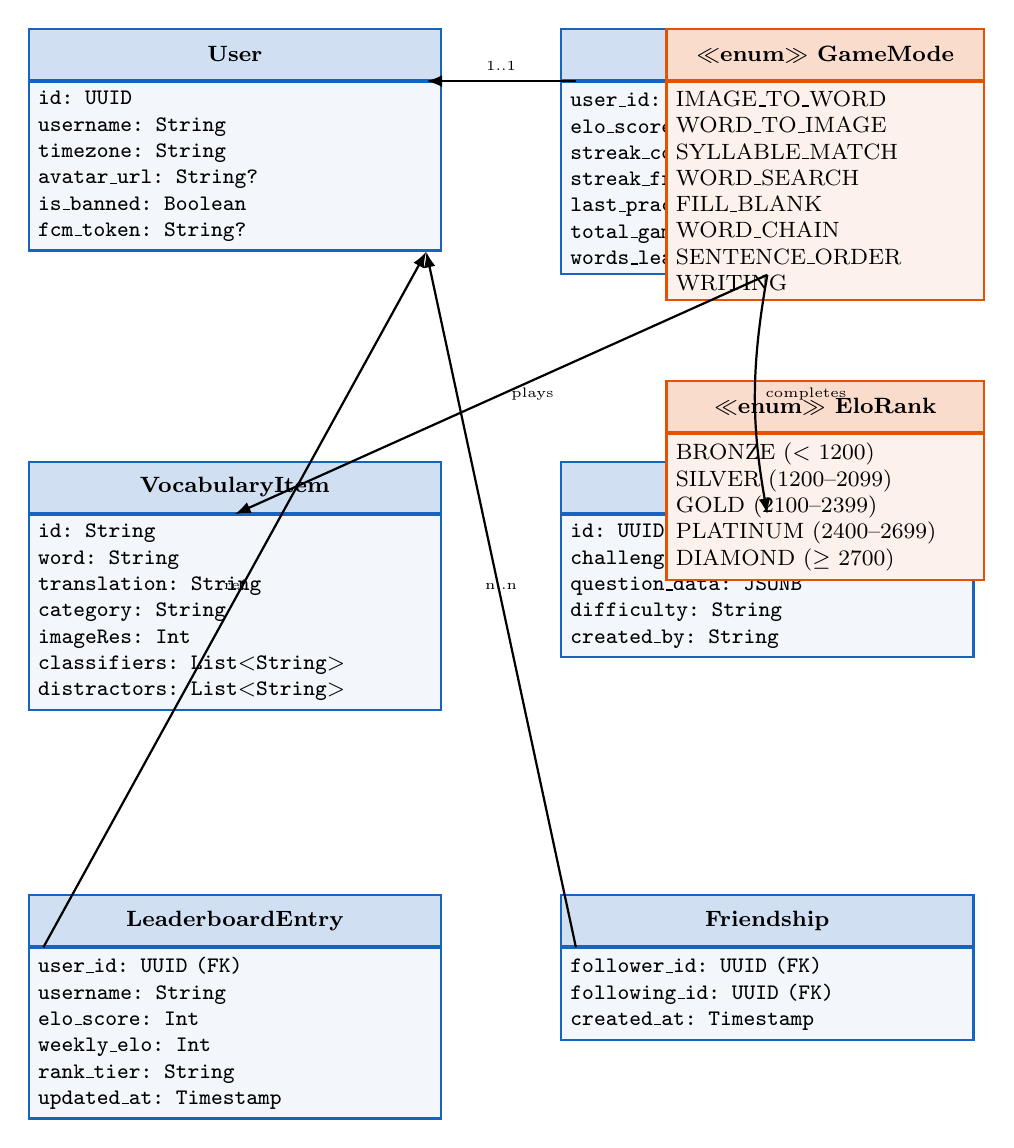
\begin{tikzpicture}[
  cls/.style={rectangle, draw=vfblue, thick, fill=vfblue!5,
    text width=5.0cm, font=\footnotesize},
  hdr/.style={rectangle, draw=vfblue, thick, fill=vfblue!20,
    text width=5.0cm, align=center, font=\footnotesize\bfseries,
    minimum height=0.65cm},
  enm/.style={rectangle, draw=vforange, thick, fill=vforange!8,
    text width=3.8cm, font=\footnotesize},
  enh/.style={rectangle, draw=vforange, thick, fill=vforange!20,
    text width=3.8cm, align=center, font=\footnotesize\bfseries,
    minimum height=0.65cm},
  comp/.style={-diamond, thick},
  agg/.style={-open diamond, thick},
  ass/.style={-{Latex[length=2mm]}, thick},
  node distance=0.0cm
]

% ---- User ----
\node[hdr] (uhdr) at (0,0) {User};
\node[cls, below=of uhdr] (ubody) {
  \texttt{id: UUID}\\
  \texttt{username: String}\\
  \texttt{timezone: String}\\
  \texttt{avatar\_url: String?}\\
  \texttt{is\_banned: Boolean}\\
  \texttt{fcm\_token: String?}
};

% ---- UserProgress ----
\node[hdr, right=1.5cm of uhdr] (uphdr) {UserProgress};
\node[cls, below=of uphdr] (upbody) {
  \texttt{user\_id: UUID (FK)}\\
  \texttt{elo\_score: Int}\\
  \texttt{streak\_count: Int}\\
  \texttt{streak\_freeze\_count: Int}\\
  \texttt{last\_practice\_date: Date?}\\
  \texttt{total\_games: Int}\\
  \texttt{words\_learned: JSONB}
};

% ---- VocabularyItem ----
\node[hdr] (vhdr) at (0,-5.5) {VocabularyItem};
\node[cls, below=of vhdr] (vbody) {
  \texttt{id: String}\\
  \texttt{word: String}\\
  \texttt{translation: String}\\
  \texttt{category: String}\\
  \texttt{imageRes: Int}\\
  \texttt{classifiers: List$<$String$>$}\\
  \texttt{distractors: List$<$String$>$}
};

% ---- DailyChallenge ----
\node[hdr, right=1.5cm of vhdr] (dchdr) {DailyChallenge};
\node[cls, below=of dchdr] (dcbody) {
  \texttt{id: UUID}\\
  \texttt{challenge\_date: Date}\\
  \texttt{question\_data: JSONB}\\
  \texttt{difficulty: String}\\
  \texttt{created\_by: String}
};

% ---- LeaderboardEntry ----
\node[hdr] (lhdr) at (0,-11.0) {LeaderboardEntry};
\node[cls, below=of lhdr] (lbody) {
  \texttt{user\_id: UUID (FK)}\\
  \texttt{username: String}\\
  \texttt{elo\_score: Int}\\
  \texttt{weekly\_elo: Int}\\
  \texttt{rank\_tier: String}\\
  \texttt{updated\_at: Timestamp}
};

% ---- Friendship ----
\node[hdr, right=1.5cm of lhdr] (fhdr) {Friendship};
\node[cls, below=of fhdr] (fbody) {
  \texttt{follower\_id: UUID (FK)}\\
  \texttt{following\_id: UUID (FK)}\\
  \texttt{created\_at: Timestamp}
};

% ---- GameMode enum ----
\node[enh] (gmhdr) at (7.5,-0) {$\ll$enum$\gg$ GameMode};
\node[enm, below=of gmhdr] (gmbody) {
  IMAGE\_TO\_WORD\\
  WORD\_TO\_IMAGE\\
  SYLLABLE\_MATCH\\
  WORD\_SEARCH\\
  FILL\_BLANK\\
  WORD\_CHAIN\\
  SENTENCE\_ORDER\\
  WRITING
};

% ---- EloRank enum ----
\node[enh, below=1cm of gmbody] (erhdr) {$\ll$enum$\gg$ EloRank};
\node[enm, below=of erhdr] (erbody) {
  BRONZE ($<$ 1200)\\
  SILVER (1200--2099)\\
  GOLD (2100--2399)\\
  PLATINUM (2400--2699)\\
  DIAMOND ($\geq$ 2700)
};

% ---- Relationships ----
\draw[ass] ([xshift=2mm]upbody.north west) -- node[above,font=\tiny]{1..1} ([xshift=-2mm]ubody.north east);
\draw[ass] ([xshift=2mm]lbody.north west) -- node[above,font=\tiny]{ref} ([xshift=-2mm]ubody.south east);
\draw[ass] ([xshift=2mm]fbody.north west) -- node[above,font=\tiny]{n..n} ([xshift=-2mm]ubody.south east);
\draw[ass] (upbody.south) -- node[right,font=\tiny]{plays} (vbody.north);
\draw[ass] (upbody.south) to[bend right=10] node[right,font=\tiny]{completes} (dcbody.north);

\end{tikzpicture}
\caption{Domain model chính của VietForces (Android data models + Supabase schema).}
\end{figure}

\subsection{Kiến trúc lớp Android (Layer Diagram)}

\begin{figure}[H]
\centering
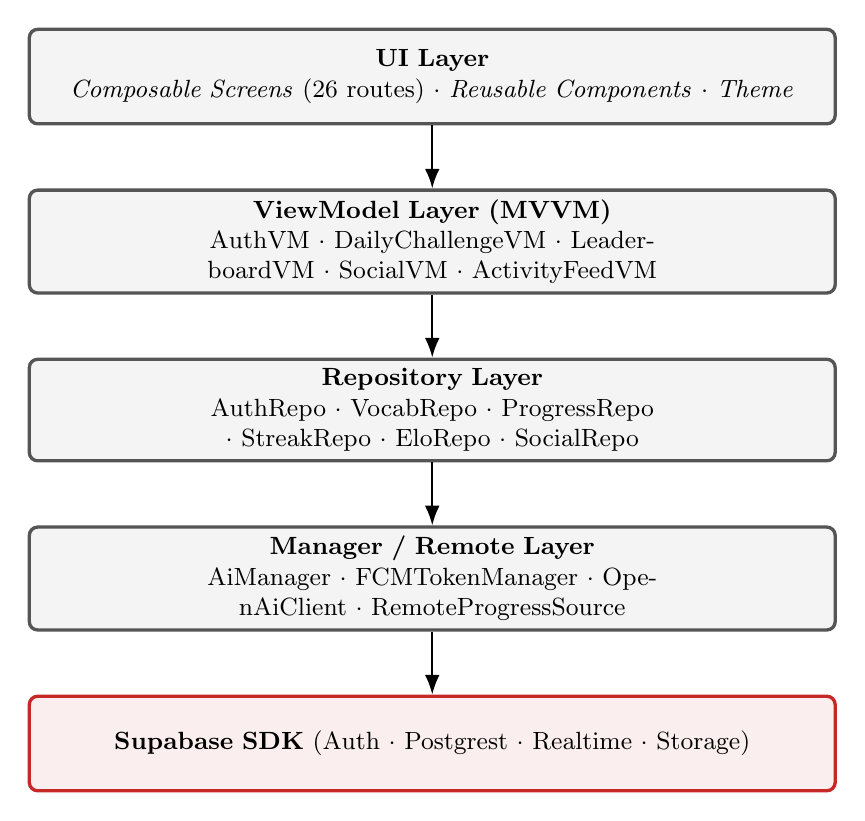
\begin{tikzpicture}[node distance=0.8cm]
  \node[layer, text width=10cm, minimum height=1.2cm] (ui)
    {\textbf{UI Layer}\\
     \textit{Composable Screens} (26 routes) $\cdot$ \textit{Reusable Components} $\cdot$ \textit{Theme}};
  \node[layer, text width=10cm, minimum height=1.2cm, below=of ui] (vm)
    {\textbf{ViewModel Layer (MVVM)}\\
     AuthVM $\cdot$ DailyChallengeVM $\cdot$ LeaderboardVM $\cdot$ SocialVM $\cdot$ ActivityFeedVM};
  \node[layer, text width=10cm, minimum height=1.2cm, below=of vm] (repo)
    {\textbf{Repository Layer}\\
     AuthRepo $\cdot$ VocabRepo $\cdot$ ProgressRepo $\cdot$ StreakRepo $\cdot$ EloRepo $\cdot$ SocialRepo};
  \node[layer, text width=10cm, minimum height=1.2cm, below=of repo] (mgr)
    {\textbf{Manager / Remote Layer}\\
     AiManager $\cdot$ FCMTokenManager $\cdot$ OpenAiClient $\cdot$ RemoteProgressSource};
  \node[cloud, text width=10cm, minimum height=1.2cm, below=of mgr] (supa)
    {\textbf{Supabase SDK} (Auth $\cdot$ Postgrest $\cdot$ Realtime $\cdot$ Storage)};

  \draw[ar] (ui)   -- (vm);
  \draw[ar] (vm)   -- (repo);
  \draw[ar] (repo) -- (mgr);
  \draw[ar] (mgr)  -- (supa);
\end{tikzpicture}
\caption{Kiến trúc phân lớp của Android app (MVVM + Repository + Hilt).}
\end{figure}

% =====================================================================
\section{Kiến trúc phần mềm (Software Architecture)}
\label{sec:architecture}

\emph{Phần này được generate từ mã nguồn thực tế và đã được kiểm tra, xác nhận
phản ánh đúng kiến trúc đang chạy.}

\subsection{Tổng quan hệ thống}

VietForces là hệ thống đa nền tảng gồm 4 thành phần chia sẻ một Supabase backend duy nhất:

\begin{figure}[H]
\centering
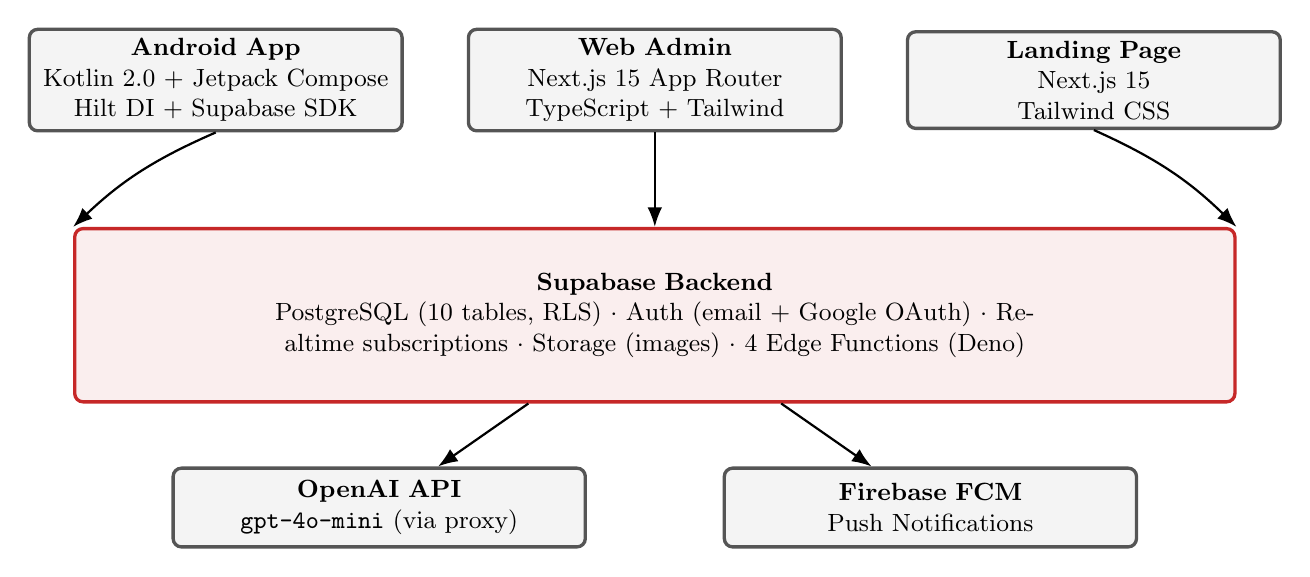
\begin{tikzpicture}[node distance=0.7cm and 1.0cm]
  \node[layer, text width=4.5cm] (android) {\textbf{Android App}\\Kotlin 2.0 + Jetpack Compose\\Hilt DI + Supabase SDK};
  \node[layer, text width=4.5cm, right=0.8cm of android] (admin) {\textbf{Web Admin}\\Next.js 15 App Router\\TypeScript + Tailwind};
  \node[layer, text width=4.5cm, right=0.8cm of admin] (landing) {\textbf{Landing Page}\\Next.js 15\\Tailwind CSS};

  \node[cloud, text width=14.5cm, minimum height=2.2cm,
        below=1.2cm of admin] (supabase)
    {\textbf{Supabase Backend}\\
     PostgreSQL (10 tables, RLS) $\cdot$ Auth (email + Google OAuth) $\cdot$
     Realtime subscriptions $\cdot$ Storage (images) $\cdot$ 4 Edge Functions (Deno)};

  \node[layer, text width=5cm, below=0.8cm of supabase, xshift=-3.5cm] (openai)
    {\textbf{OpenAI API}\\\texttt{gpt-4o-mini} (via proxy)};
  \node[layer, text width=5cm, below=0.8cm of supabase, xshift=3.5cm] (fcm)
    {\textbf{Firebase FCM}\\Push Notifications};

  \draw[ar] (android.south) to[bend right=10] (supabase.north west);
  \draw[ar] (admin.south) -- (supabase.north);
  \draw[ar] (landing.south) to[bend left=10] (supabase.north east);
  \draw[ar] (supabase) -- (openai);
  \draw[ar] (supabase) -- (fcm);
\end{tikzpicture}
\caption{Kiến trúc tổng thể hệ thống VietForces.}
\end{figure}

\subsection{Android App — MVVM + Repository}

Android app theo pattern MVVM (Model–View–ViewModel) kết hợp Repository pattern và
Hilt Dependency Injection:

\begin{description}[leftmargin=2cm]
  \item[\textbf{UI Layer}] 26 Composable screen routes, 6 ViewModel classes, các
        reusable Component composables.
  \item[\textbf{ViewModel Layer}] \texttt{@HiltViewModel} classes, expose
        \texttt{StateFlow<UiState>}. Async work trong \texttt{viewModelScope.launch\{\}}.
  \item[\textbf{Repository Layer}] Interface + \texttt{Impl} classes — abstraction trên
        Supabase SDK. Trả \texttt{Result<T>}, không throw lên ViewModel.
  \item[\textbf{Remote / Manager Layer}] \texttt{OpenAiClient} (HTTP), \texttt{AiManager}
        (prompt builder + JSON parser), \texttt{FCMTokenManager}, \texttt{PreferencesManager}.
\end{description}

\subsection{Supabase Backend}

\begin{table}[H]
\centering
\begin{tabular}{@{}p{4cm}p{9cm}@{}}
\toprule
\textbf{Bảng / Function} & \textbf{Mục đích} \\
\midrule
\texttt{users} & Thông tin người dùng, kế thừa \texttt{auth.users} \\
\texttt{user\_progress} & ELO, streak, từ đã học (JSONB), last\_practice\_date \\
\texttt{leaderboard} & Snapshot ELO cho realtime ranking (all-time + weekly) \\
\texttt{daily\_challenges} & Dữ liệu thử thách hàng ngày (JSONB question\_data) \\
\texttt{daily\_completions} & Bản ghi hoàn thành daily challenge (dedup) \\
\texttt{streak\_history} & Lịch sử ngày luyện tập để render heatmap \\
\texttt{activity\_feed} & Sự kiện hoạt động của bạn bè (follows, completions) \\
\texttt{friendships} & Quan hệ follow (asymmetric) \\
\texttt{notification\_preferences} & Bật/tắt từng loại notification của user \\
\texttt{admin\_schema} & Bảng cấu hình admin dashboard \\
\midrule
\texttt{calculate\_elo()} & SECURITY DEFINER — tính ELO delta, cập nhật leaderboard \\
\texttt{update\_streak()} & SECURITY DEFINER — xử lý streak logic + freeze \\
\texttt{award\_daily\_bonus()} & SECURITY DEFINER — cộng ELO, tạo daily\_completion \\
\midrule
\textbf{Edge Function} & \\
\texttt{openai-proxy} & Relay AI call từ Android đến OpenAI, giữ API key server-side \\
\texttt{generate-daily-challenge} & Tạo daily challenge mới lúc 00:00 UTC (pg\_cron) \\
\texttt{send-streak-reminder} & Gửi FCM push notification nhắc học (~19:00 UTC) \\
\texttt{refresh-streak-freeze} & Nạp lại 1 streak freeze cho mọi user mỗi tuần \\
\bottomrule
\end{tabular}
\caption{Cấu trúc Supabase backend — bảng, function, và Edge Functions.}
\end{table}

\subsection{Web Admin Dashboard}

\begin{itemize}
  \item \textbf{Framework:} Next.js 15 App Router, TypeScript, Tailwind CSS
  \item \textbf{Auth:} Supabase Auth với middleware guard (\texttt{middleware.ts})
  \item \textbf{Tính năng:} Vocabulary CRUD + image upload, User management (ban/unban),
        Analytics dashboard (DAU, retention), Daily challenge scheduling
  \item \textbf{Deploy:} Vercel
\end{itemize}

% =====================================================================
\section{AI Integration (Advanced Feature)}
\label{sec:ai}

\emph{Đây là phần nổi bật nhất của đề tài — tích hợp LLM (OpenAI gpt-4o-mini)
để cá nhân hoá trải nghiệm học và tạo tình huống hội thoại thực tế.}

\subsection{Kiến trúc AI}

AI layer trong VietForces được thiết kế theo nguyên tắc \textbf{``grade locally first,
call AI only when necessary''} để giữ app nhanh và tiết kiệm chi phí.

\begin{figure}[H]
\centering
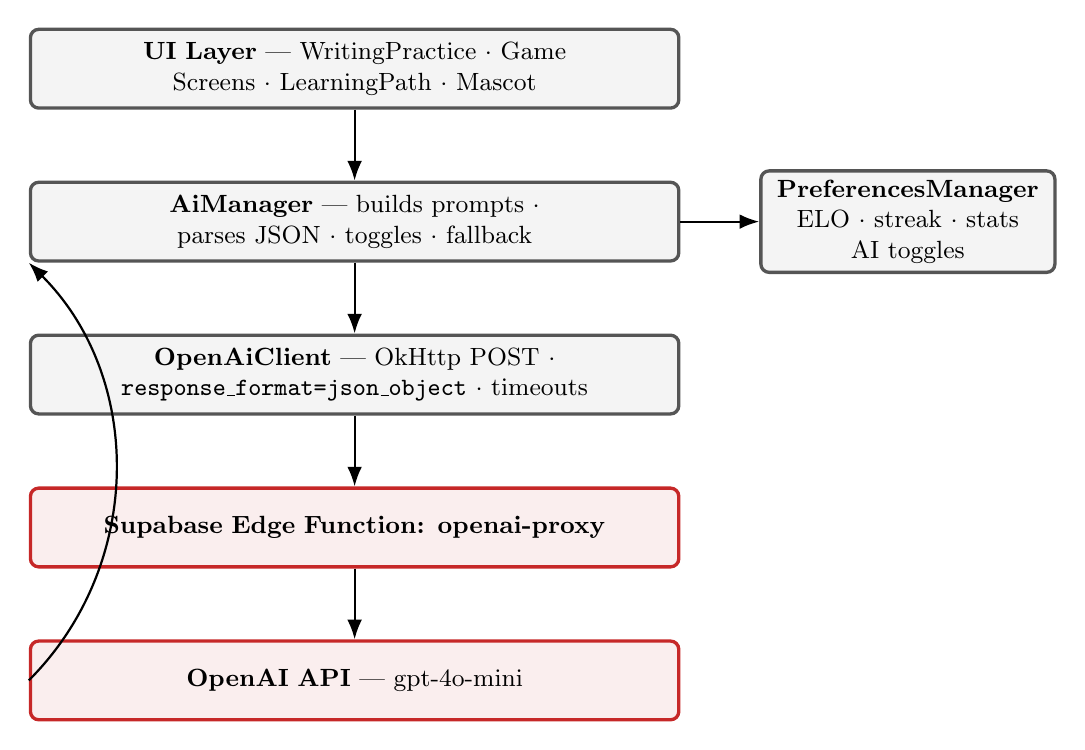
\begin{tikzpicture}[node distance=0.9cm]
  \node[layer, text width=8cm] (ui)   {\textbf{UI Layer} — WritingPractice $\cdot$ Game Screens $\cdot$ LearningPath $\cdot$ Mascot};
  \node[layer, text width=8cm, below=of ui] (mgr) {\textbf{AiManager} — builds prompts $\cdot$ parses JSON $\cdot$ toggles $\cdot$ fallback};
  \node[layer, text width=8cm, below=of mgr] (cli) {\textbf{OpenAiClient} — OkHttp POST $\cdot$ \texttt{response\_format=json\_object} $\cdot$ timeouts};
  \node[layer, text width=3.5cm, right=1.0cm of mgr] (pref) {\textbf{PreferencesManager}\\ELO $\cdot$ streak $\cdot$ stats\\AI toggles};
  \node[cloud, text width=8cm, below=of cli] (proxy) {\textbf{Supabase Edge Function: openai-proxy}};
  \node[cloud, text width=8cm, below=of proxy] (oai)  {\textbf{OpenAI API} — gpt-4o-mini};

  \draw[ar] (ui) -- (mgr);
  \draw[ar] (mgr) -- (cli);
  \draw[ar] (cli) -- (proxy);
  \draw[ar] (proxy) -- (oai);
  \draw[ar] (oai.west) to[bend right=45] (mgr.south west);
  \draw[ar] (mgr) -- (pref);
\end{tikzpicture}
\caption{Kiến trúc AI layer — Android App $\rightarrow$ Edge Function Proxy $\rightarrow$ OpenAI.}
\end{figure}

\subsection{5 tính năng AI}

\begin{enumerate}
  \item \textbf{Writing Grading} — AI chấm đoạn văn ngắn tiếng Việt: điểm 0–10, chỉ lỗi
        (ngữ pháp, dấu thanh, từ vựng), gợi ý bản viết lại.
  \item \textbf{Open-answer Grading} — Chấm câu trả lời theo nghĩa (không phải string
        equality): chấp nhận câu thiếu dấu hoặc diễn đạt khác nhưng đúng ý.
  \item \textbf{Mascot Reactions} — Linh vật gà trống phản hồi tự nhiên sau mỗi câu
        trả lời (throttle 6 giây, instant string + AI upgrade).
  \item \textbf{Personalised Learning Path} — AI phân tích stats người học
        (ELO, accuracy per mode, words hay sai) và đề xuất lộ trình luyện tập ưu tiên.
  \item \textbf{AI Roleplay Conversation Tutor} — Chat đa lượt với AI đóng vai
        nhân vật Việt Nam: người bán phở, tài xế Grab, người bán hàng chợ, v.v.
        AI nói tiếng Việt tự nhiên nhưng đơn giản; có gợi ý câu học viên có thể nói tiếp.
\end{enumerate}

\subsection{Bảo mật và chi phí}

\begin{itemize}
  \item \textbf{API key an toàn:} OpenAI key chỉ tồn tại trong Supabase Environment Variables —
        không có trong APK hay source code.
  \item \textbf{Graceful fallback:} Mọi AI call đều có \texttt{AiCallResult.Error} path;
        app không crash khi AI lỗi.
  \item \textbf{Chi phí thấp:} \texttt{gpt-4o-mini} $\approx$ \$0.00003/call, throttle
        mascot 6 giây, các tính năng khác là user-triggered.
  \item \textbf{Structured output:} \texttt{response\_format = json\_object} đảm bảo
        AI trả JSON hợp lệ; \texttt{AiManager} parse tolerant.
\end{itemize}

% =====================================================================
\section{Ảnh chụp màn hình (UI Screenshots)}
\label{sec:screenshots}

\emph{Thêm ảnh thực tế vào thư mục \texttt{report/images/} với tên file đúng như trong README.
Phần này sẽ hiển thị ảnh khi compile.}

Để thêm ảnh vào báo cáo, đặt file ảnh vào \texttt{report/images/} và bỏ comment phần
\texttt{\textbackslash includegraphics} tương ứng bên dưới.

% ---- Hướng dẫn: bỏ comment % ở các dòng includegraphics khi đã có ảnh ----
\begin{figure}[H]
\centering
% \includegraphics[width=0.3\textwidth]{images/screenshot_home.png}
% \hfill
% \includegraphics[width=0.3\textwidth]{images/screenshot_game_image_to_word.png}
% \hfill
% \includegraphics[width=0.3\textwidth]{images/screenshot_game_fill_blank.png}
\fbox{\parbox{0.3\textwidth}{\centering\vspace{3cm}\small[Home Screen]\vspace{3cm}}}
\hfill
\fbox{\parbox{0.3\textwidth}{\centering\vspace{3cm}\small[ImageToWord Game]\vspace{3cm}}}
\hfill
\fbox{\parbox{0.3\textwidth}{\centering\vspace{3cm}\small[FillBlank Game]\vspace{3cm}}}
\caption{Màn hình chính và hai game modes (thay bằng screenshot thực tế).}
\end{figure}

\begin{figure}[H]
\centering
% \includegraphics[width=0.3\textwidth]{images/screenshot_leaderboard.png}
% \hfill
% \includegraphics[width=0.3\textwidth]{images/screenshot_daily_challenge.png}
% \hfill
% \includegraphics[width=0.3\textwidth]{images/screenshot_ai_roleplay.png}
\fbox{\parbox{0.3\textwidth}{\centering\vspace{3cm}\small[Leaderboard]\vspace{3cm}}}
\hfill
\fbox{\parbox{0.3\textwidth}{\centering\vspace{3cm}\small[Daily Challenge]\vspace{3cm}}}
\hfill
\fbox{\parbox{0.3\textwidth}{\centering\vspace{3cm}\small[AI Roleplay]\vspace{3cm}}}
\caption{Leaderboard real-time, Daily Challenge, và AI Roleplay.}
\end{figure}

\begin{figure}[H]
\centering
% \includegraphics[width=0.9\textwidth]{images/screenshot_admin.png}
\fbox{\parbox{0.9\textwidth}{\centering\vspace{3cm}\small[Web Admin Dashboard]\vspace{3cm}}}
\caption{Web Admin Dashboard — vocabulary management, user management, analytics.}
\end{figure}

% =====================================================================
\section{Video Demo}
\label{sec:demo}

\begin{tcolorbox}[colback=boxbg, colframe=vfblue, title={\textbf{Hướng dẫn Demo}},
  fonttitle=\bfseries]
\begin{enumerate}
  \item \textbf{Kịch bản demo đề xuất:}
    \begin{enumerate}[label=\alph*.]
      \item Mở app, đăng nhập tài khoản.
      \item Chơi game mode \textit{ImageToWord} và \textit{Roleplay} (AI tính năng nổi bật).
      \item Mở Daily Challenge — hoàn thành và xem streak +1.
      \item Mở Leaderboard — xem real-time update.
      \item Mở Writing Practice — viết đoạn văn và xem AI feedback.
      \item Mở Web Admin — thêm một từ vựng mới.
    \end{enumerate}
  \item \textbf{Thời lượng đề xuất:} 3–5 phút.
  \item \textbf{Upload video lên:} Google Drive / YouTube (unlisted) và đính kèm link vào báo cáo.
\end{enumerate}
\end{tcolorbox}

\vspace{0.5cm}
\textbf{Link video demo:} \underline{\hspace{8cm}} (điền vào khi có)

% =====================================================================
\section{Tính năng nổi bật (Advanced Features)}
\label{sec:advanced}

\begin{enumerate}
  \item \textbf{AI Integration (OpenAI gpt-4o-mini):}
    \begin{itemize}
      \item 5 tính năng AI: Writing Grading, Open-answer Grading, Mascot Reactions,
            Learning Path, Roleplay Conversation Tutor.
      \item Mọi AI call trả structured JSON — không phụ thuộc vào text parsing fragile.
      \item Graceful fallback hoàn toàn — app chạy được dù không có internet.
    \end{itemize}

  \item \textbf{Server-authoritative ELO + Real-time Leaderboard:}
    \begin{itemize}
      \item ELO tính hoàn toàn server-side bởi PostgreSQL function (SECURITY DEFINER).
      \item Supabase Realtime WebSocket subscription — leaderboard cập nhật không cần F5.
    \end{itemize}

  \item \textbf{Gamification đầy đủ:}
    \begin{itemize}
      \item 8 game modes học từ vựng với 100+ từ phân loại theo 8 chủ đề.
      \item Hệ thống streak với Streak Freeze (auto-apply khi bỏ 1 ngày).
      \item Daily Challenge server-generated, đổi mỗi ngày lúc 00:00 UTC.
      \item ELO ranking với 5 tier (Bronze $\to$ Diamond).
    \end{itemize}

  \item \textbf{Smart Push Notifications (FCM):}
    \begin{itemize}
      \item Supabase Edge Function gửi FCM push nhắc học theo timezone của từng user.
      \item Người dùng tự cài đặt bật/tắt từng loại notification.
    \end{itemize}

  \item \textbf{Social + Activity Feed:}
    \begin{itemize}
      \item Asymmetric follow system (như Twitter).
      \item Activity feed hiển thị hoạt động của bạn bè.
      \item Friends tab trong leaderboard.
    \end{itemize}
\end{enumerate}

\end{document}
